% Created 2018-06-09 Sat 11:12
% Intended LaTeX compiler: pdflatex
\documentclass[11pt]{article}
\usepackage[utf8]{inputenc}
\usepackage[T1]{fontenc}
\usepackage{graphicx}
\usepackage{grffile}
\usepackage{longtable}
\usepackage{wrapfig}
\usepackage{rotating}
\usepackage[normalem]{ulem}
\usepackage{amsmath}
\usepackage{textcomp}
\usepackage{amssymb}
\usepackage{capt-of}
\usepackage{hyperref}
\usepackage{placeins}
\usepackage[margin=0.5in]{geometry}
\usepackage[parfill]{parskip}
\date{\today}
\title{}
\hypersetup{
 pdfauthor={},
 pdftitle={},
 pdfkeywords={},
 pdfsubject={},
 pdfcreator={Emacs 26.0.91 (Org mode 9.1.13)}, 
 pdflang={English}}
\begin{document}

\tableofcontents

\section{Ressourcen, Prozesse und Ziele betrieblicher Leistungserstellung}
\label{sec:org65b9814}
\subsection{Leistungsbereich(Produktion)}
\label{sec:org1d09ca4}
\begin{center}
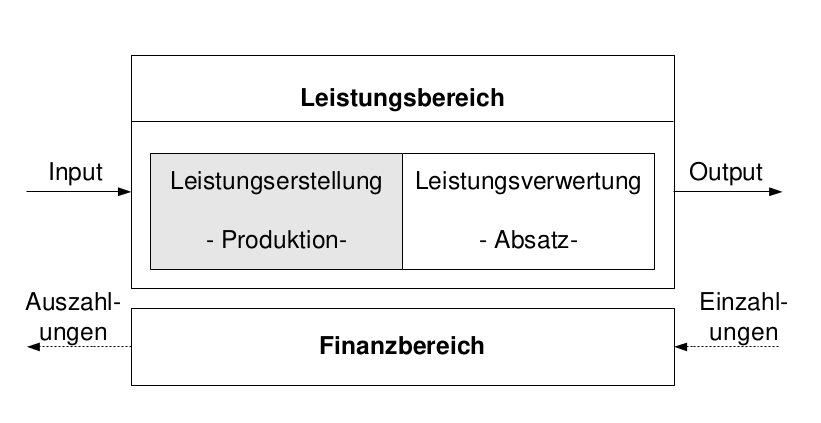
\includegraphics[width=250px]{./pictures/leistungsbereich_prod.png}
\end{center} 

\FloatBarrier

\subsubsection{Produktion, Produktionsfaktoren, Produktionswirtschaft}
\label{sec:orga469479}
\textbf{Produktion} = der industrielle Abbau von Material, dessen Be- und Verarbeitung und die Ausführung von Dienstleistungen; ist die methodische Umwandlung von Produktionsfaktoren in Produkte im Rahmen von bestimmten Produktionsverfahren

\textbf{Produktionsfaktoren} = sind die in der Produktion eingesetzen materiellen und immateriellen Güter, durch deren Gebrauch \& Verbrauch neue Sachgüter \& Dienstleistungen (Services) entsehen; Produktionsmittel nach Gutenberg = Betriebsmittel, Werkstoffe, (objektbezogene/dispositive) Arbeitsleistungen

\textbf{Produktionswirtschaft} = Aufgabe der Produktionswirtschaft ist die Planung, Durchführung \& Kontrolle der industriellen Leistungserstellung, um wirtschaftliche Produktionsstrukturen zu erreichen \& zu sichern
\subsection{Finanzierungsbereich}
\label{sec:orgb748580}

\begin{center}
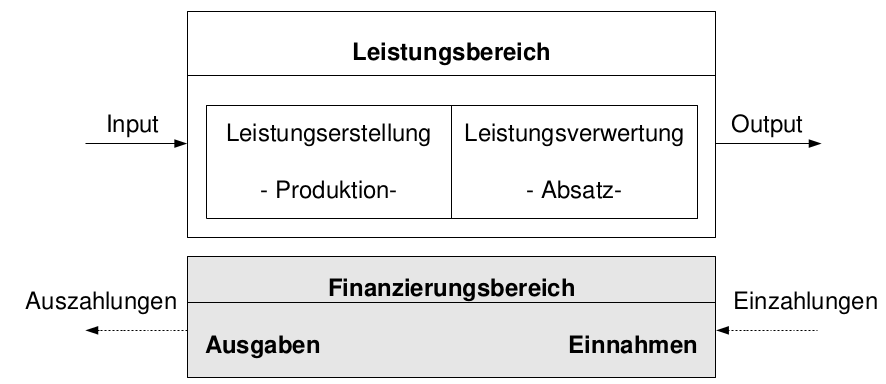
\includegraphics[width=250px]{./pictures/finanzierungsbereich.png}
\end{center} 

Finanzierung ist sowas wie eine Beanspruchung unter Versprechen auf Erfüllung
\begin{itemize}
\item betriebliche Finanzierung umfasst Beschaffung und Rückzahlung finanzieller Mittel und damit verbunden die Gestaltung der Beziehungen zw Unternehmen und Kapitalgebern
\item \emph{Finanzierungsmaßnahmen} beginnen mit Einzahlung an das Unternehmen, worauf Auszahlungen in späteren Perioden Folgen (Passivseite der Bilanz)
\item Gesamtheit aller Finanzmittel eines Unternehmens wird als Kapital bezeichnet
\end{itemize}

Investition ist sowas wie Verzicht in der Hoffnung auf Belohnung
\begin{itemize}
\item zielgerichteter Einsatz von finanziellen Mitteln zur Erwirtschaftung von Erträgen
\item \emph{Investitionsmaßnahmen} beginnen mit Auszahlung an das Unternehmen, auf die Einzahlungen in späteren Perioden folgen (Aktivseite der Bilanz)
\end{itemize}
bild von seite 12 iwo hin

\subsubsection{Finanzwirtschaft \& Zahlungsströme}
\label{sec:org6fb75c3}
\textbf{Monetärer Kapitalbegriff} = im Unternehmen eingesetzte Zahlungsmittel

\textbf{Finanzierung} ist die Kapitalbeschaffung für die jeweilige Unternehmung. Die \textbf{Finanzwirtschaft} umfasst diese Kapitalbeschaffung und -verwendung in der Unternehmung. Zu den finanzwirtschaftlichen Zielen gehört die Erreichung eines \emph{finanzwirtschaftlichen Gleichgewichts}, das bedeutet die Sicherung der dispositiven Liquidität, sowie die Sicherung der strukturellen Liquidität.

Die Funktion des \textbf{Finanzmanagements} ist die zielgerichtete Gestaltung der betrieblichen Finanzwirtschaft. Dazu zählt hauptsächlich die aktive Gestaltung der Kapitalzuführung \& des Kapitalentzugs.

\paragraph{Monetäre Zielgrößen}\\
\begin{itemize}
\item Zahlungsmittelbestand = Kassenbestand, Guthaben bei Kreditinstituren; Einzahlung, Auszahlung
\item Geldvermögen = Zahlungsmittelbestand + Forderungen - Verbindlichkeiten; Einnahme, Ausgabe
\item Gesamtvermögen = Gewinn + Verlustrechnung; Ertrag, Aufwand
\item Betriebsnotwendiges Vermögen = Kosten- und Leistungsrechnung; Ertrag, Aufwand
\end{itemize}


\subsection{Gegenstandbereich \& Ziele betrieblicher Leistungserstellung}
\label{sec:orgf01890d}
\subsubsection{Betriebliche Leistungserstellung als Kombinationsprozess (Gutenberg)}
\label{sec:orgd5365d1}
"\emph{Die Ergiebigkeit des Faktoreinsatzes in den  Betrieben ist einmal von der Beschaffenheit der Faktoren selbst und zum anderen von ihrer Kombination abhängig.
Es gilt deshalb zu untersuchen, welche Umstände es sind, die den produktiven Beitrag bestimmen, den sie im Rahmen einer Faktorkombination zu leisten imstande sind.}" (Gutenberg 1975)

Beim Input der betrieblichen Leistungserstellung unterscheidet man zwischen Potential- und Repetierfaktoren
\begin{center}
\begin{tabular}{ll}
 & Repetierfaktoren (Verbrauch)\\
Charakteristik & gehen im Produktionsprozess physisch \& mengenmäßig unter\\
Bestimmung des Werteverzehrs & i.d.R leicht zu bewerten \& zuzuordnen\\
Teilbarkeit & i.d.R beliebig teilbar\\
Beispiele & Werkstoffe, Energie\\
\end{tabular}
\end{center}

\begin{center}
\begin{tabular}{ll}
 & Potentialfaktoren (Gebrauch/Bestand)\\
Charakteristik & stellen längerfristig verfügbare Nutzungspotentiale bereit\\
Bestimmung des Werteverzehrs & schwer bestimmtbar, Unsicher in der Zuordnung zB technischer Verschleiß\\
Teilbarkeit & i.d.R nicht beliebig teilbar\\
Beispiele & materiell: maschinelle Anlagen, Gebäude; immateriell: Rechte (Patente, Lizenzen), technische Informationen (Software)\\
\end{tabular}
\end{center}

\begin{figure}[htbp]
\centering
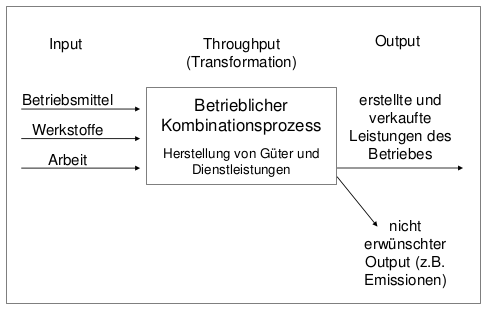
\includegraphics[width=250px]{./pictures/produktion_als_kombpr.png}
\caption{Produktion als Kombinationsprozess}
\end{figure} 

\FloatBarrier

\subsubsection{Ziele \& Zielkonflikte produktionswirtschaftlicher Betätigung}
\label{sec:org49cc1ae}
\end{document}
